\documentclass[12pt]{article}

\usepackage[utf8]{inputenc}
\usepackage[russian]{babel}
\usepackage{amsmath}
\usepackage{setspace}

\usepackage{caption}
\usepackage{subcaption}
\usepackage{float}
\usepackage{graphicx}
\graphicspath{ {./images/} }

\usepackage{geometry}
 \geometry{
 a4paper,
 left=20mm,
 right=20mm,
 top=20mm,
 bot=20mm,
 }

\begin{document}

\begin{titlepage}
\begin{center}
    {\small НАЦИОНАЛЬНЫЙ ИССЛЕДОВАТЕЛЬСКИЙ УНИВЕРСИТЕТ ИТМО} \\
    {\small Факультет систем управления и робототехники} \\
    \vspace*{10\baselineskip}
    {\LARGEЭлектроника и схемотехника} \\
    \ \\
    \begin{spacing}{1.5}
    {\large Лабораторная работа №7 \\
    Триггеры на логических элементах} \\
    \end{spacing} \\
    \ \\
    Вариант 2 \\
    \vspace*{10\baselineskip}
    \hfill {Выполнили студенты:} \\
    \hfill {Кирбаба Д.Д. R3338} \\
    \hfill {Курчавый В.В. R3338} \\
    \ \\
    \hfill {Преподаватель:} \\
    \hfill {Николаев Н.А.} \\
    \mbox{}
    \vfill {г. Санкт-Петербург\\2023}
\end{center}
\end{titlepage}

\section*{Цель работы}
Моделирование и исследование работы $JK-$, $RS-$ и $D-$триггеров в LtSpice.

\section*{Ход работы}
Вариант 2.\\
Тип триггера: синхронный $RS$-триггер на ИЛИ-НЕ.

\begin{figure}[H]
    \centering
    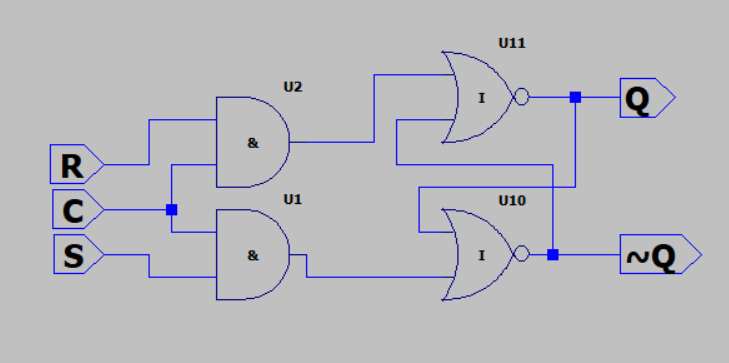
\includegraphics[width=0.7\textwidth]{scheme.png}
    \caption{Блок-схема синхронного $RS$-триггера на ИЛИ-НЕ.}
    \label{fig:scheme}
\end{figure}

\begin{figure}[H]
    \centering
    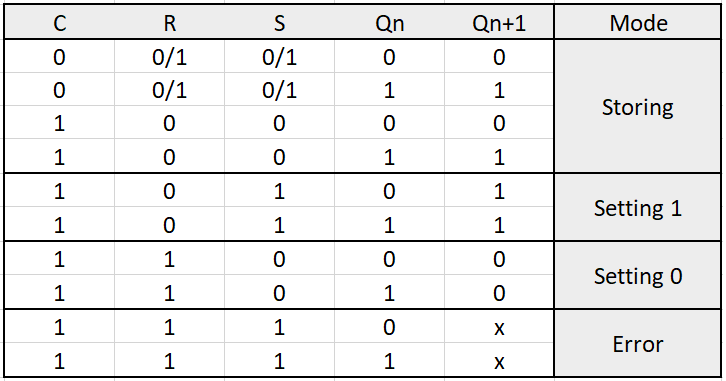
\includegraphics[width=0.7\textwidth]{state_table.png}
    \caption{Таблица состояний синхронного $RS$-триггера.}
    \label{fig:state_table}
\end{figure}

Приведем временные диаграммы для каждого из состояний:

\begin{figure}[H]
    \centering
    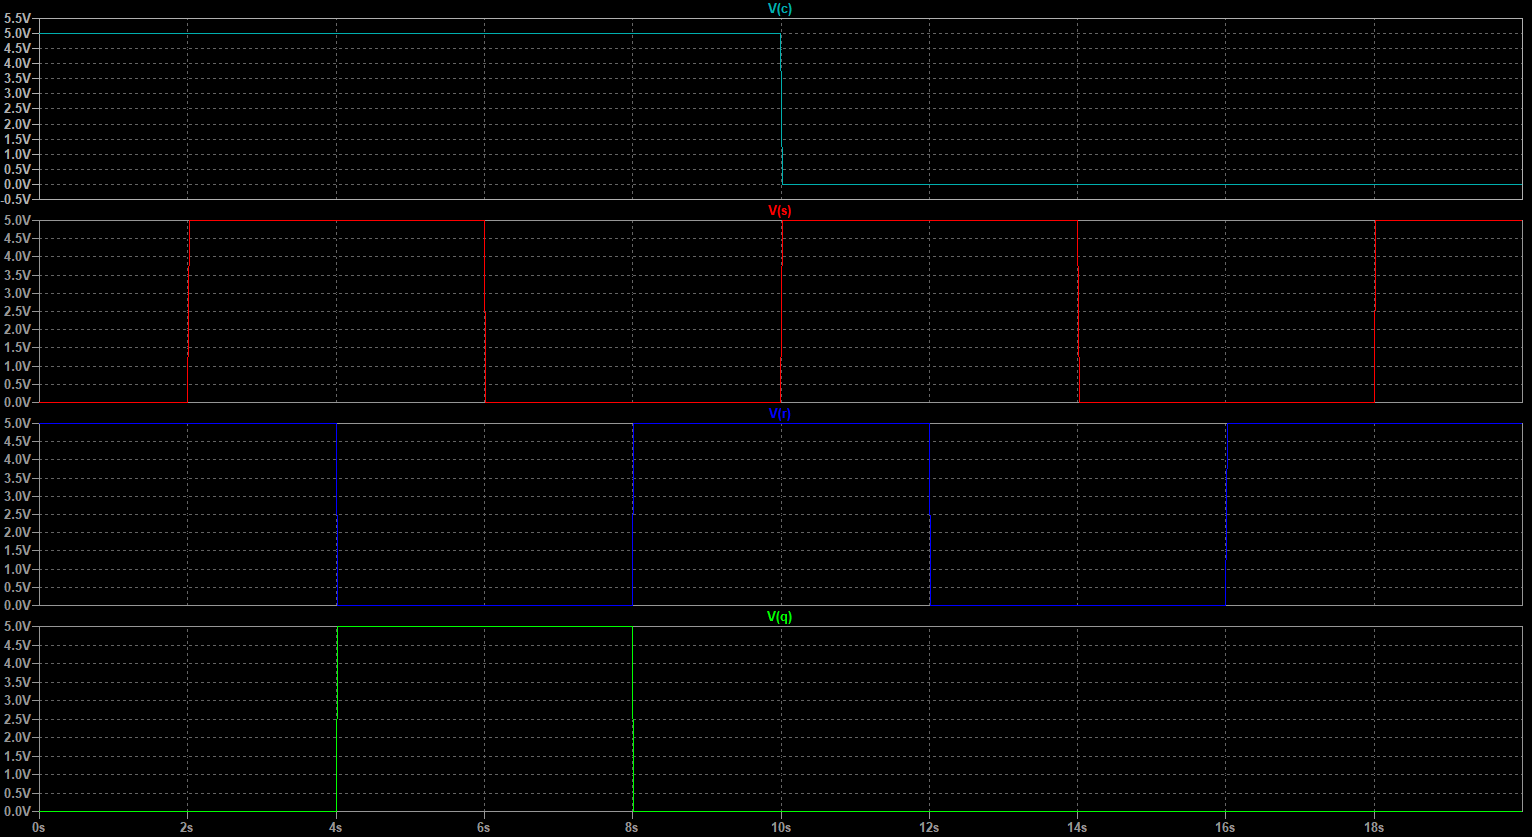
\includegraphics[width=\textwidth]{graph_0.png}
    \caption{Временная диаграмма с сохранением сигнала $0$.}
    \label{fig:graph_0}
\end{figure}

\begin{figure}[H]
    \centering
    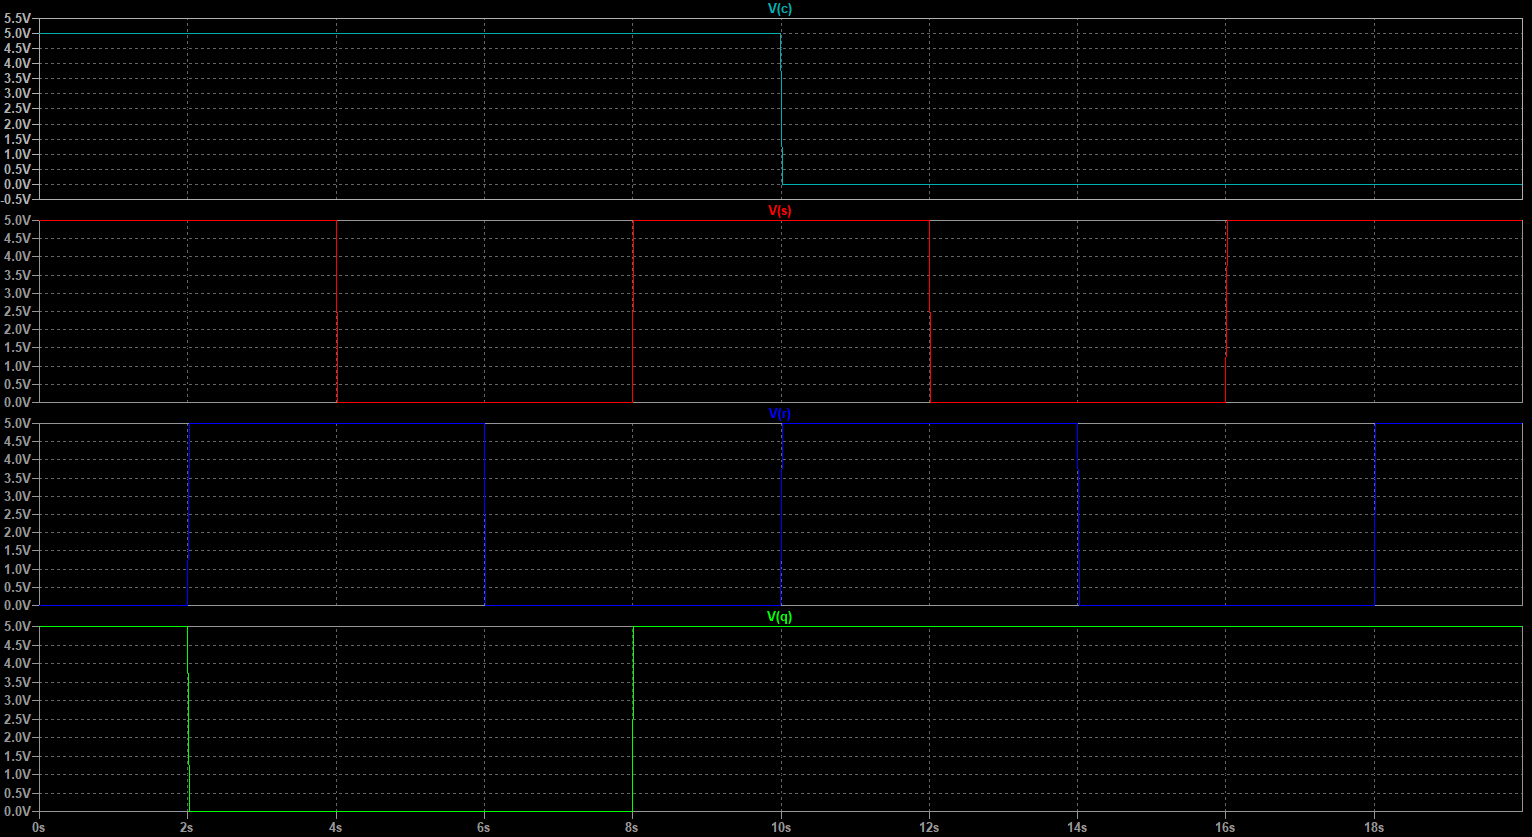
\includegraphics[width=\textwidth]{graph_1.png}
    \caption{Временная диаграмма с сохранением сигнала $1$.}
    \label{fig:graph_1}
\end{figure}

На приведенных графиках выше можем наблюдать все состояния триггера: 
\begin{itemize}
    \item установка значений $0$ и $1$ (левая половина на обоих графиках);
    \item хранение значений $0$ и $1$ при единичном сигнале $C$ (левая половина на обоих графиках);
    \item неопределенное значение (в данном случае равно всегда $1$, также наблюдается на левой половине на обоих графиках);
    \item хранение значения $0$ при нулевом сигнале $C$ (правая половина на первом графике);
    \item хранение значения $1$ при нулевом сигнале $C$ (правая половина на втором графике).
\end{itemize}

\section*{Выводы}
В данной работе изучались триггеры - электронные устройства, имеющие свойство долго находиться в одном из двух устойчивых состояний и чередовать их под воздействием внешних сигналов. Триггер имеет два состояния, которые можно обозначить $0$ и $1$, таким образом появляется возможность хранить один разряд двоичного числа. \\
\ \\
По заданному варианту, исследовалась работа синхронного $RS$-триггера. Синхронизирующий сингал необходим для избежания проблемы когда на вход триггера сигналы $SET$, $RESET$ пришли в неправильном порядке. При добавлении синхронизации триггер будет как-либо реагировать на входные сигналы только в том случае, когда на вход $C$ подана единица. В остальных случаях триггер будет находиться в режиме хранения состояния.\\
\ \\
При выполнении работы была построена блок-схема $RS$-триггера на логических элементах в базисе ИЛИ-НЕ, синхронизирующая часть была построена в базисе И-НЕ (одноко при желании можно перевести в базис ИЛИ-НЕ используя теорему двойственности). \\
Затем были выбраны такие параметры сигналов, чтобы можно было пронаблюдать каждое состояние триггера. \\
В результате, поведение выходного сигнала триггера совпало с ожидаемым, а значит работа проделана верно. 

\end{document}